\documentclass[../ClassicThesis.tex]{subfiles}
\begin{document}

%************************************************
\chapter{Curves/Deus}\label{ch:curves}
%************************************************

\section{Cutting curved shapes}

Approximating curved shapes with parts created by the laser cutter is a special challenge because only 2D shapes can be cut. There are several approaches to make the cut material bendable, for example, paper can already be bent because of the material properties, acrylic if it is heated and wood with the help of living hinges.

Theoretically, this only enables the possibility to create shapes from developable surfaces, like cylinders, but no doubly curved ones, like spheres. But since our meshes are based on triangles, which are themselves 2D, our meshes are always developable.

\section{The bent plate object}

Bent plate is a data structure we use to represent a set of plates which are connected directly or indirectly with bend connections so one bent plate could be cut as one piece. A Bent Plate consists of a set of plates. It has the method generateShape which develops the surface of the connected shapes. An other method it implements is generateBendLines.

\subsection{Function generateShape}

To generate the shape of the bent plate we first check how many plates are contained in this bent plate. If none is contained the generated shape is null. If there is just one then the shape is the shape of this plate.

If there are more then one plate in the bent plate the generation works the following way: The shapes from all plates of the bent plate are transformed using the bend matrix (see section \ref{sec:traverse-along-bend-connection}). Then they are converted into polygons of the \jsclipper{} and merged using the union function.To avoid unconnected polygons after merging caused by floating point inaccuracy we use vertex welding before merging. The resulting polygon is converted back to a shape. (see Listing \ref{lst:generateShape})

\begin{listing}[ht]
\begin{minted}[
linenos,breaklines
]{coffeescript}
generateShape: ->
    if @plates.length < 1
      @shape = null
      return
    if @plates.length is 1
      @shape = @plates[0].shape
      return
    # lay shapes into xy-plane
    polygons = @plates.map (plate) =>
      bentMatrix = plate.bentMatrix
      shape = plate.shape
      contour = @applyMatrices shape.getContour(), bentMatrix
      holes = shape.getHoles().map (hole) => @applyMatrices hole, bentMatrix
      return {contour, holes }
    # remove-doubles-fix
    weldingDistance = 0.02
    welder = new VertexWelding(weldingDistance)
    polygons.forEach (polygon) ->
      polygon.contour.forEach (vertex) ->
        correspondingVertex = welder.getCorrespondingVertex(
          {x: vertex[0], y: vertex[1], z: 0})
        vertex[0] = correspondingVertex.x
        vertex[1] = correspondingVertex.y
    # create clipping polygons
    polygons = polygons.map (polygon) ->
      return new Clipper.Polygon polygon.contour, polygon.holes
    # merge polygons
    mergedPolygon = polygons[0]
    polygons.shift()
    mergedPolygon = mergedPolygon.unionMultiple polygons
    # create shape from clipping polygon
    contour = mergedPolygon[0].getShape().map (vertex) ->
      return new THREE.Vector3 vertex[0], vertex[1], 0
    contour = new EdgeLoop contour
    holes = mergedPolygon[0].getHoles().map (hole) ->
      hole = hole.map (vertex) ->
        return new THREE.Vector3 vertex[0], vertex[1], 0
      hole = new EdgeLoop hole
      hole.hole = true
      return hole
    shape = holes
    shape.push contour
    shape = new Shape shape, new THREE.Vector3 0, 0, 1
    # set shape as shape of the bent plate
    @shape = shape
\end{minted}
\caption{Creating the transformation matrix for a plate as part of a bent plate.}
\label{lst:generateShape}
\end{listing}

\subsection{Function generateBendLines}

In the current implementation this method generates a dashed line at the connection lines between two plates in the shape of the bent plate. This helps to know where which part must be bend and also weakens the material to make it more easy to bend.

\section{General approach}

In our implementation, we use bends as joint type as an alternative to, for example, finger joints. Therefore, it is based like the finger joint generation on the plate graph. The bent plate generation is separated into two steps. First, our implementation analyses which parts can be bent. Second, it creates a flat shape from the curved parts.

\section{prerequisites creating bent plates}

Because we use bends as a connection type the bent plate creation is based on the plate graph. It uses the plates and its connections. From the plates it needs the shape, the normal and the rotation matrix to lay it into the xy-plane. From the connection the implementation needs the angle and the intersection line. Another step that have to be done before is the finger joint generation. The shapes of those have to be stored in the corresponding connection.

\section{Setting the joint type}

In this step, we try to find out which connections between two plates could be a bending joint so that the resulting shape of the connected plates is flattable without overlaps. An example for a model where its surface is not devlopable without overlaps is shown in Figure \ref{fig:overlaps}.

\begin{figure}[h]
  \centering
  \begin{subfigure}[b]{0.49\textwidth}
    \centering
    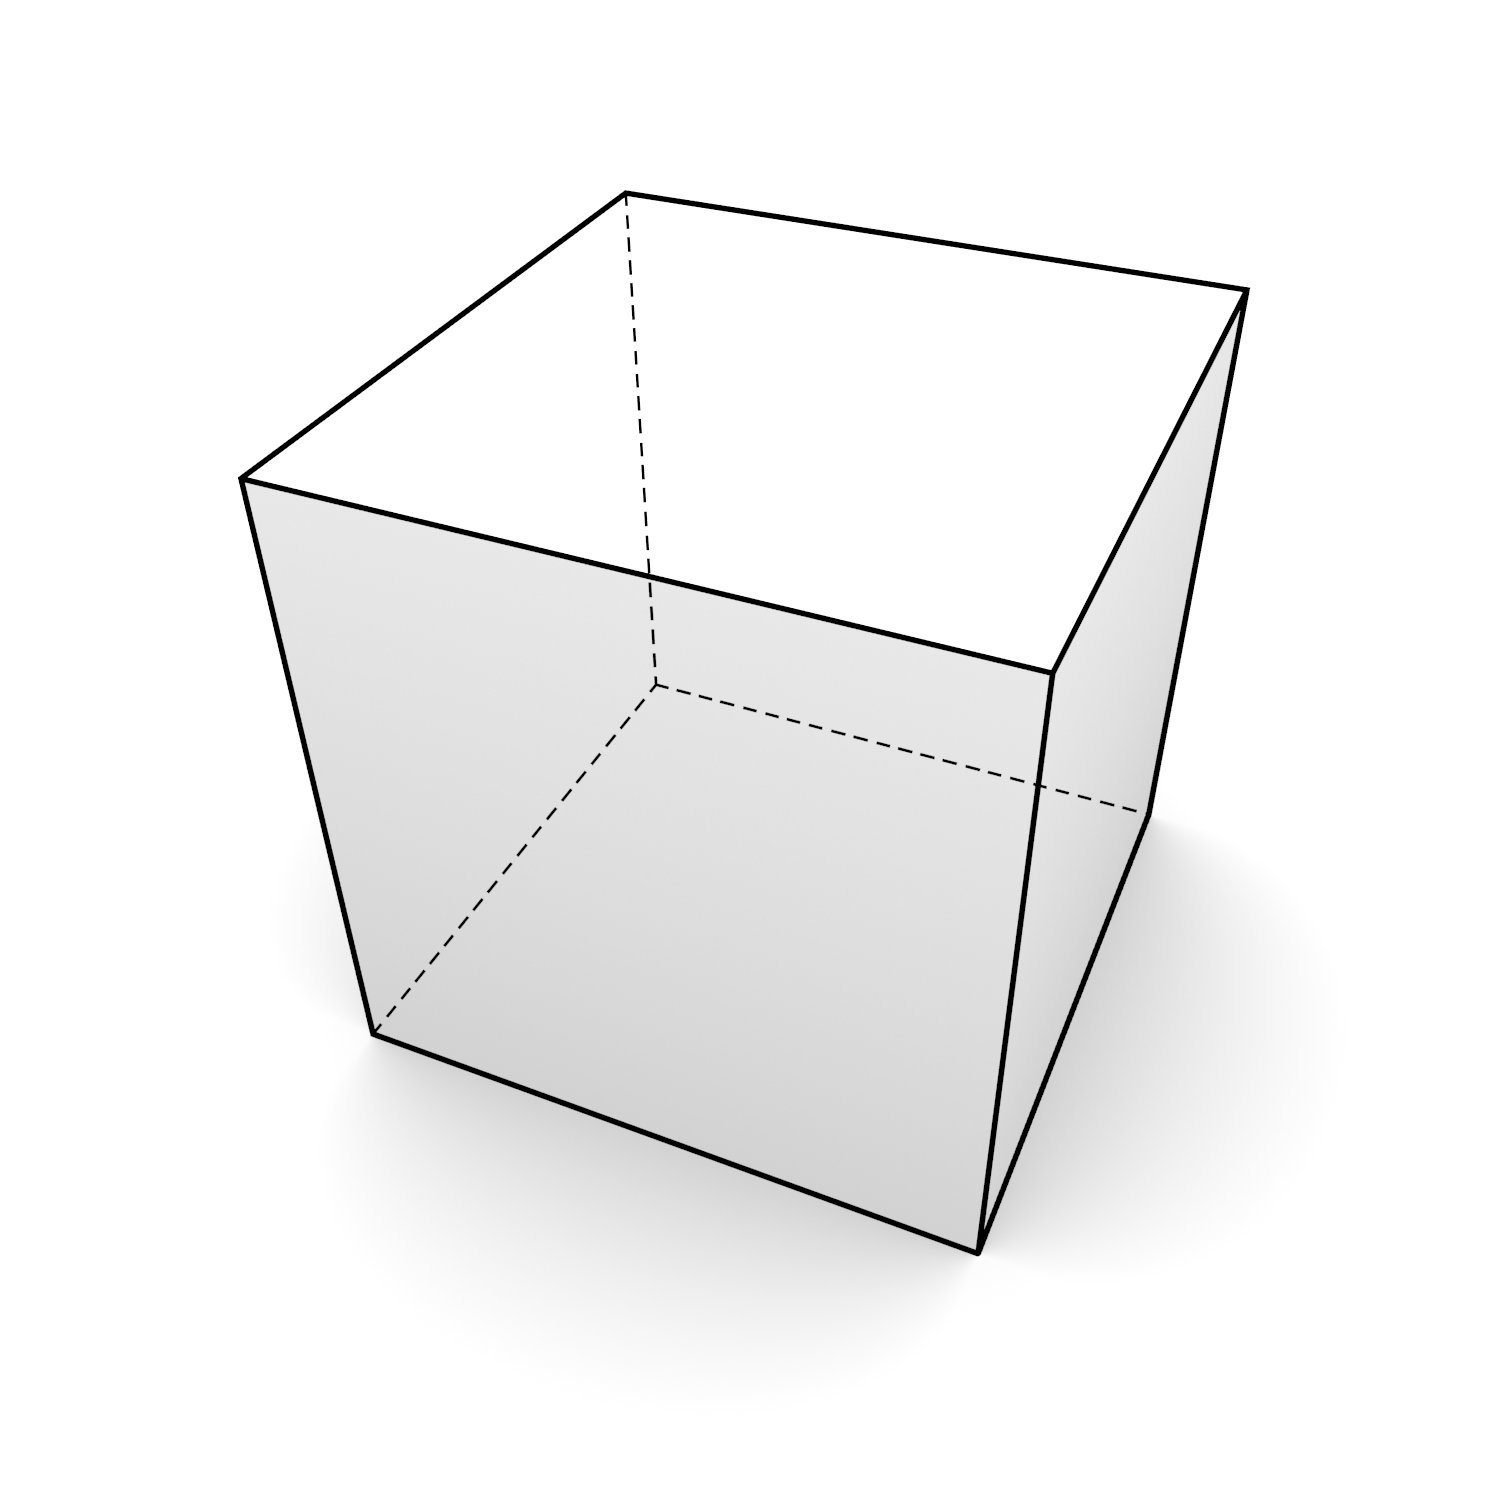
\includegraphics[width=\textwidth]{07-no_overlaps}
    \caption{A cubes surface can be developed without overlaps.}
    \label{fig:overlaps:no-3d}
  \end{subfigure}
  \begin{subfigure}[b]{0.49\textwidth}
    \centering
    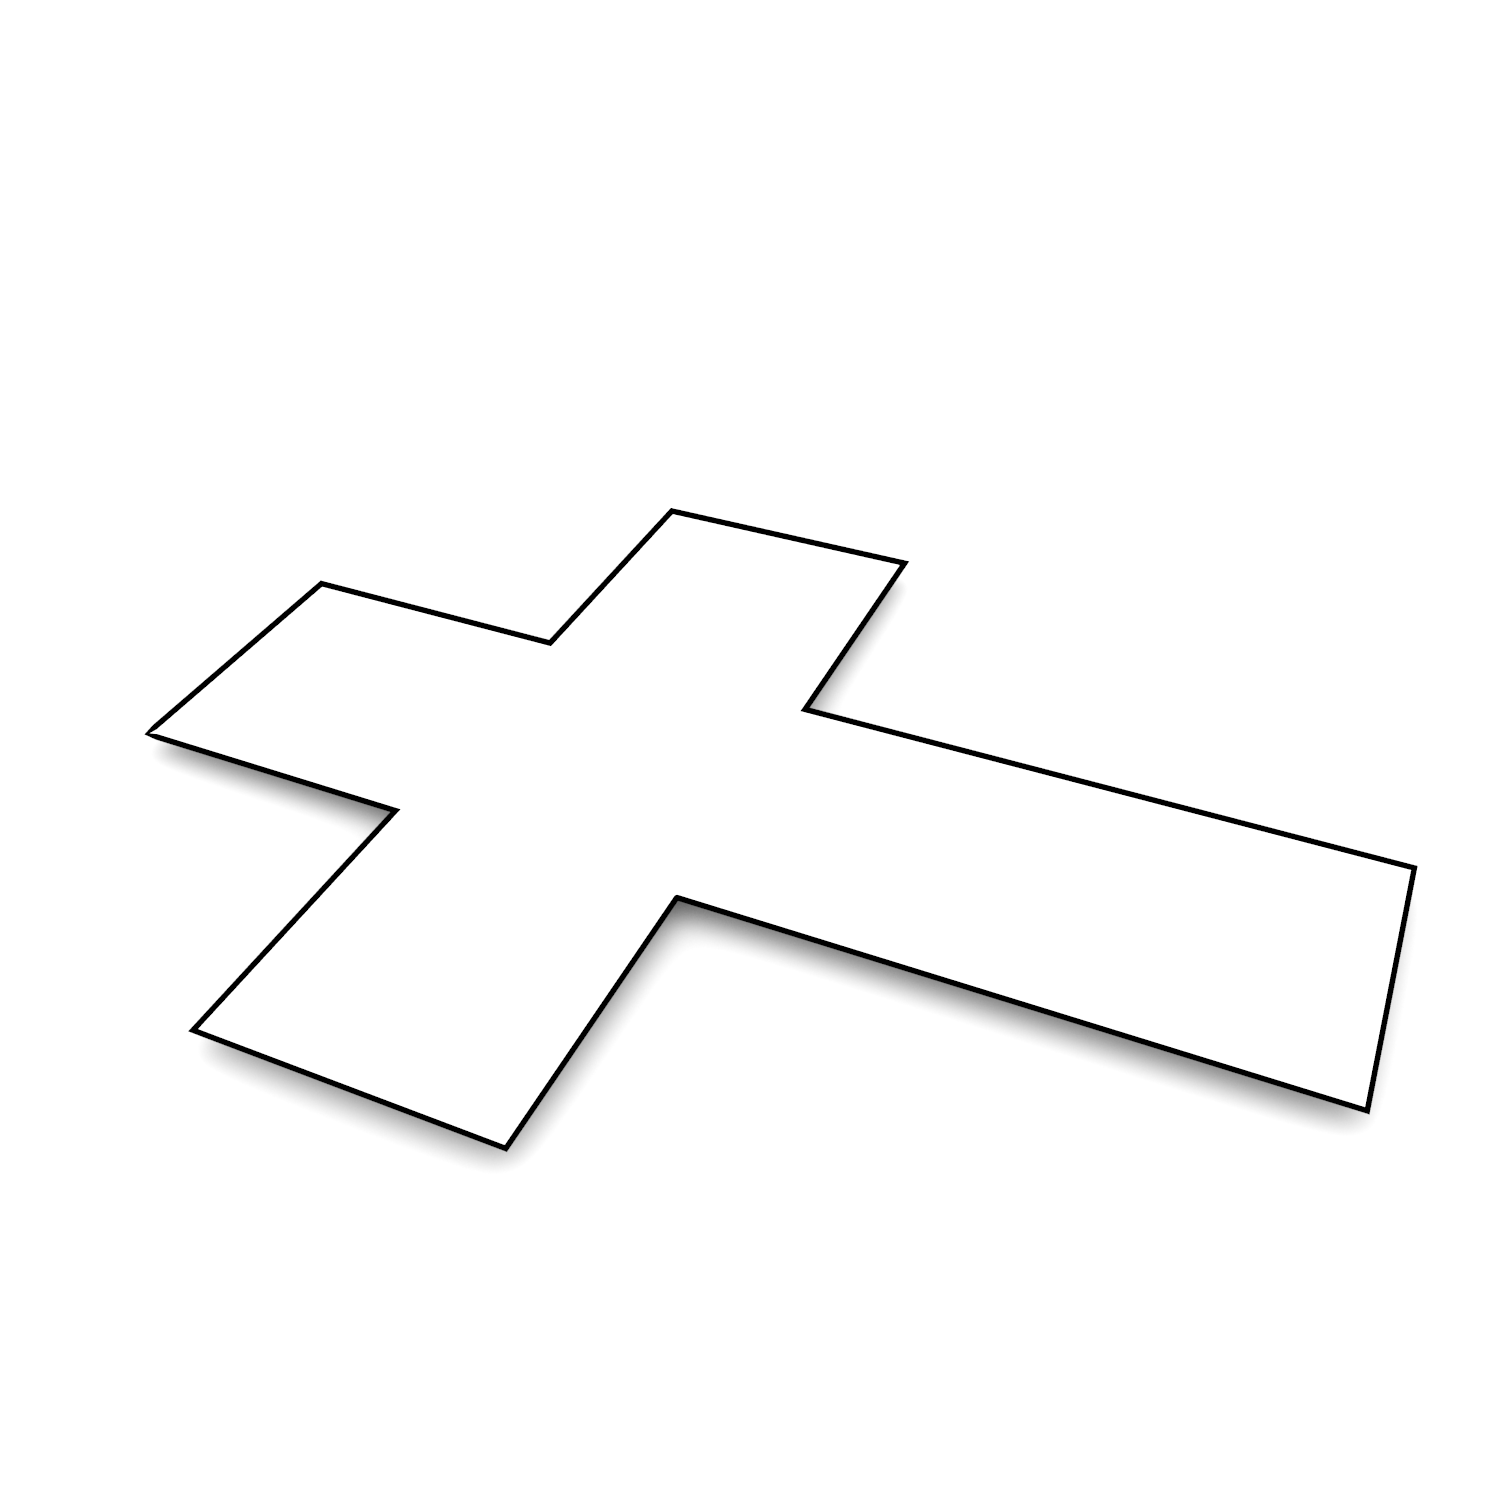
\includegraphics[width=1\textwidth]{07-no_overlaps_2d}
    \caption{One possible developed surface of a cube.}
    \label{fig:overlapsh:no-2d}
  \end{subfigure}
  \begin{subfigure}[b]{0.49\textwidth}
    \centering
    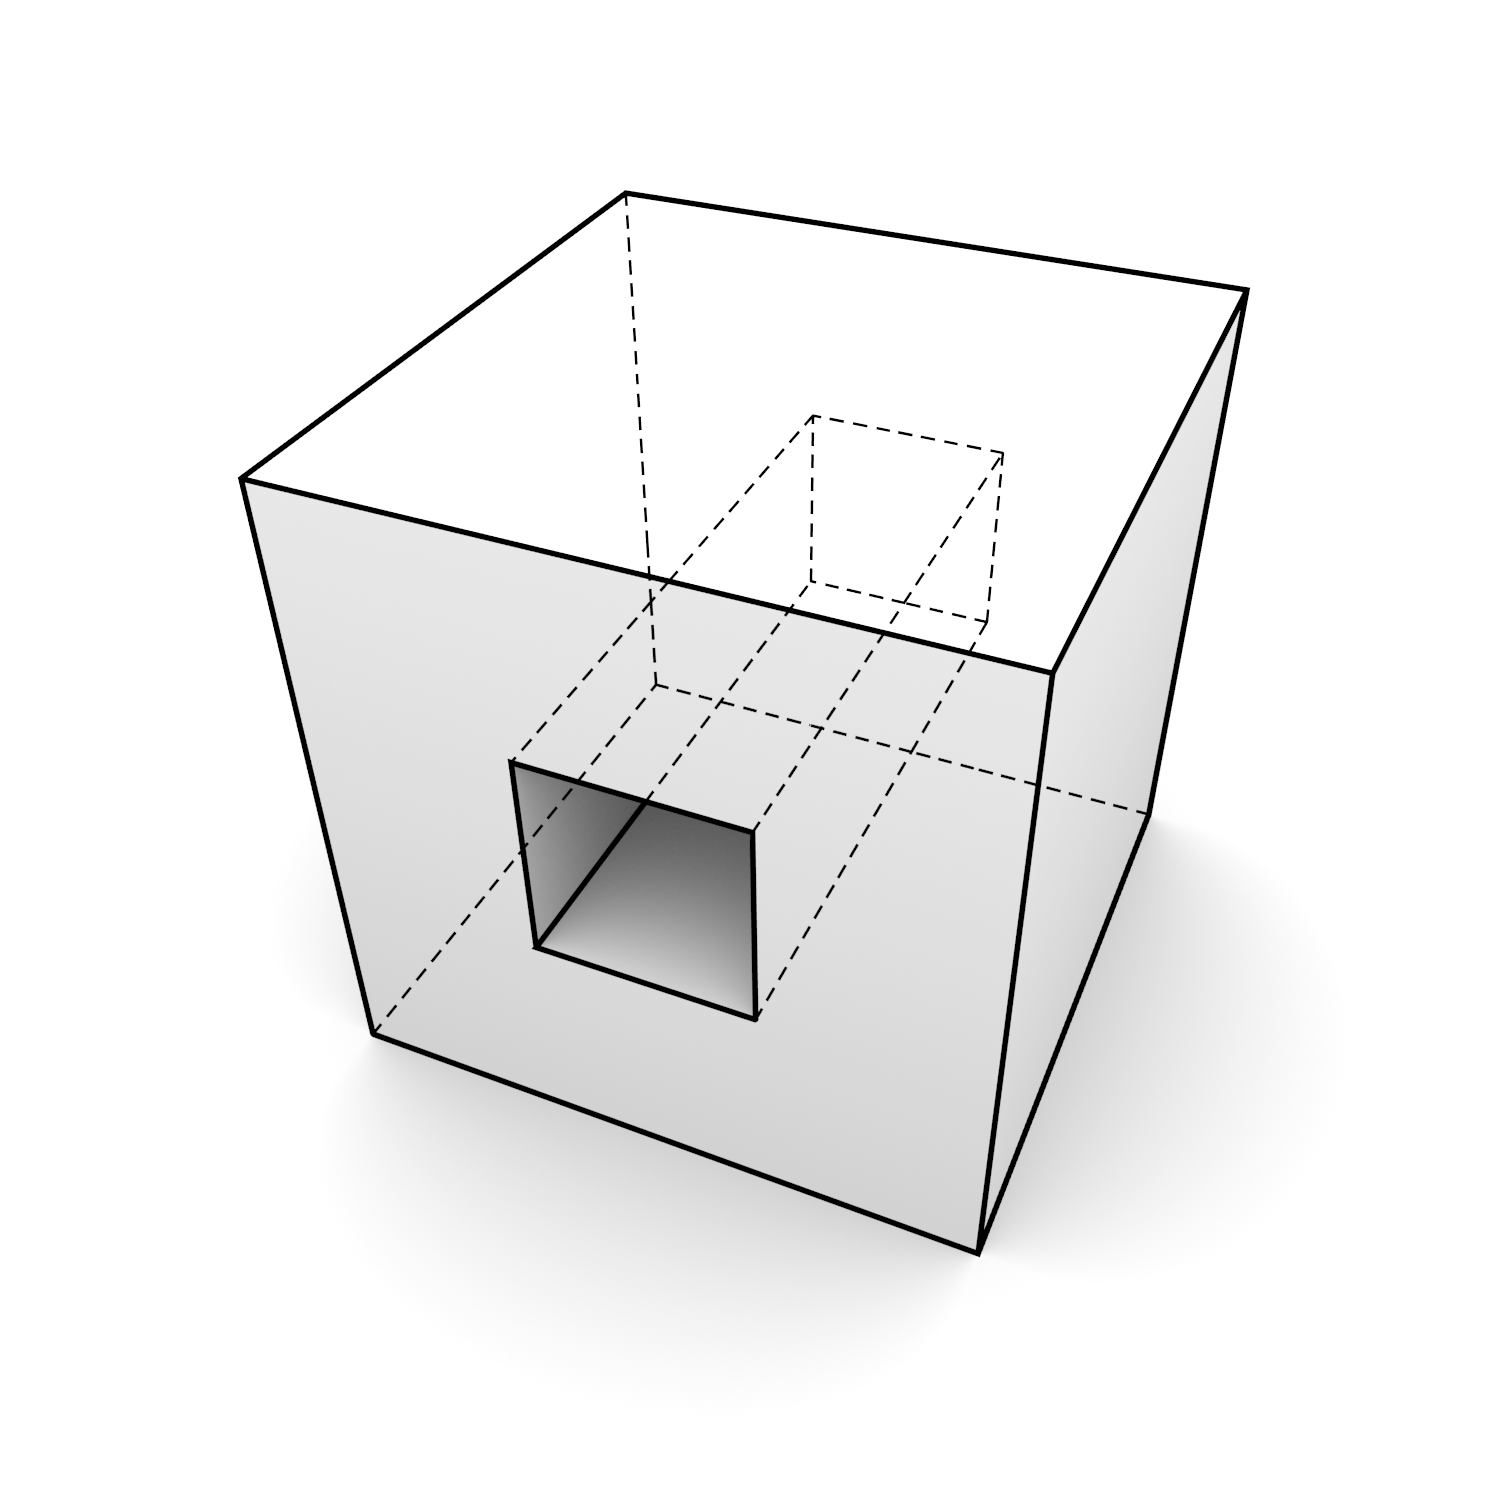
\includegraphics[width=\textwidth]{07-overlaps}
    \caption{The surface of a cube with hole can not be developed without overlaps.}
    \label{fig:overlaps:some-3d}
  \end{subfigure}
  \begin{subfigure}[b]{0.49\textwidth}
    \centering
    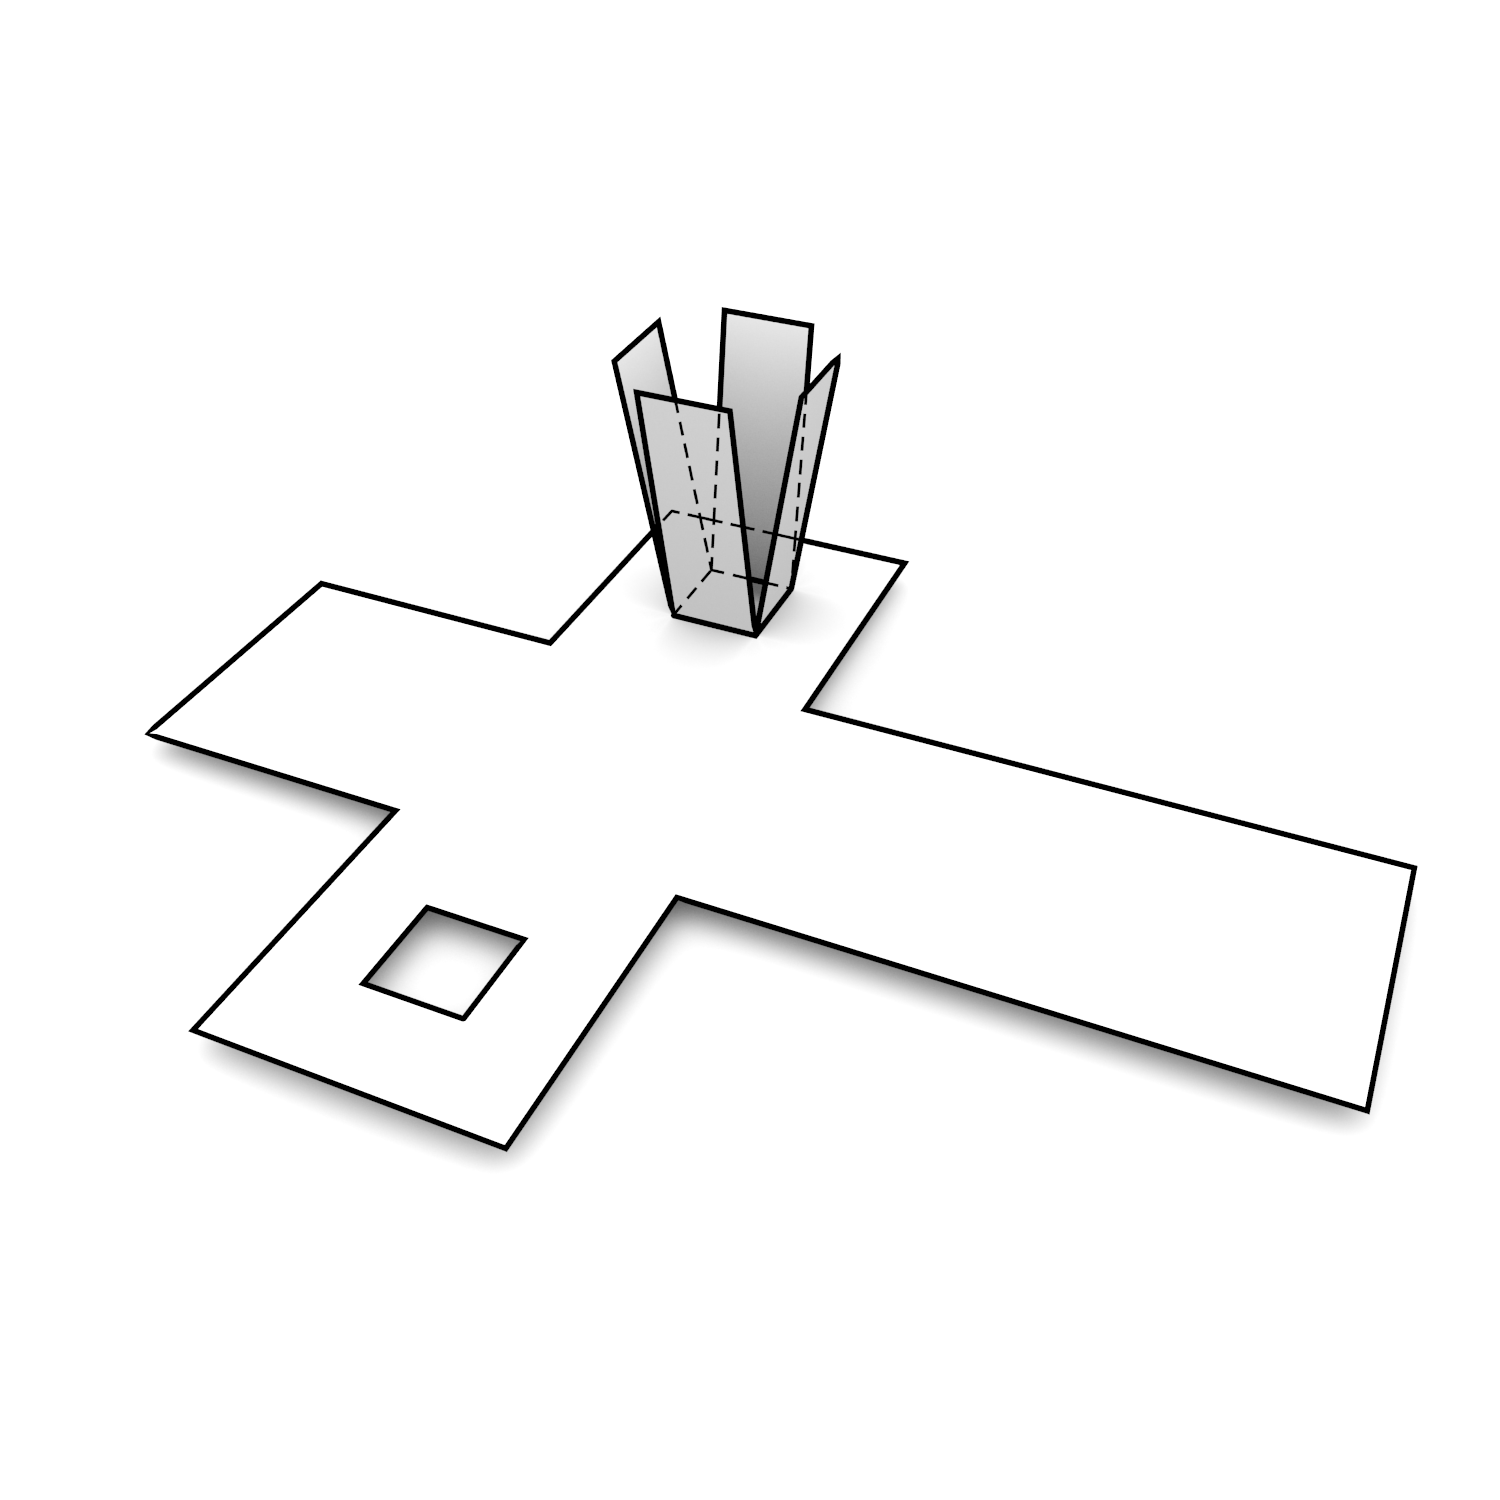
\includegraphics[width=1\textwidth]{07-overlaps_2d}
    \caption{The shapes inside the hole will always overlap some part of the developed surface.}
    \label{fig:overlaps:some-2d}
  \end{subfigure}
  \caption{A scene graph showing a box, composed of plates.}
  \label{fig:overlaps}
\end{figure}

To do so, we start with one plate and check for all of its connections:
\begin{itemize}
\item Is this connection not set already?
\item Is the connection angle close enough to 180\textdegree{} which means bending the material this far is possible? (What near enough means depends on the used material)
\item Is it possible to add the shape of the connected plate without overlapping the already existing shape?
\end{itemize}
If the answer is yes to all, the connected plate is added to this plate and they form a bent plate. If the connection type not set but the angle does not match or there are overlaps the type is set to finger joint.

This is repeated for all the connections of the bent plate until they are all set to be a bending or a finger joint. If after this some plates are not assigned to a bent plate the process is repeated for one of these until none is left.

%shorten this sentence:
To check if a plate could be added to an existing bent plate two shapes are created. The first one is the union of the bent plate shape and all of its finger joint shapes except for the connection to the new plate. The second is the union of the shape of the new plate and its finger joint shapes except for the connection to the bent plate.

Then we calculate the intersection of this two. If the result is empty there are no overlaps, the plate can be safely added to the bent plate and the connection annotated as a bending joint.

%If one of the conditions is not fulfilled the connection can not be a bend and is annotated as finger joint.

\section{Building the bent plates}
%TODO find subsection title
For building the bent plates our implementation starts with one plate of the plate graph and traverses the graph along the marked bend connections. This way all directly or indirectly connected plates (via bend connections) are collected into a array. From these plates one bent plate is created. If there are plates in the plate graph that are not added to a bent plate, at least a one plate bent plate, it is repeated with one left plate until no plate is left.

\subsection{Traverse along bend connection}
\label{sec:traverse-along-bend-connection}

While traversing along the bend connections the transformations matrices for the plates are calculated.

For the first plate the matrix is already known. It is the rotation matrix of its shape to rotate it into the xy-plane.

For the other plates it is important to make sure that they keep touching with the connected plate while laying them into the xy-plane. Therefore the bend angle must be calculated which is 180\textdegree{} minus the angle between the connected plates, which is already known from the plate graph creation.

Additionally, the bend axis is determined building the cross product of the two normals of the connected plates. This way the axis does not only lie at the right place but also points in the right direction (which it would not if only the connection line between the two plates is used).

This axis has to be transformed to lay in the xy-plane at the edge of the previous plate. To do so our implementation uses the start point of the intersection line and end point created by adding the axis vector to the start point. These two points are transformed by the be transformation matrix of the previous plate. From the transformed points the final axis is determined by subtracting the end point form the start point.

The angle and the axis are used to create the rotation matrix to lay the plate in the same plane like the previous onr.

Because the rotation matrix only rotates around the point of origin, two translation matrices are created. First, one for translating the plate to the origin to perform the rotation there. Second, one to translate the plate back to the connection edge.

To get the final transformation matrix the transformation matrix of the previous plate is multiplied by the first translation matrix, the rotation matrix and finally the second translation matrix.

\begin{figure}[h]
  \centering
  \begin{subfigure}[b]{0.49\textwidth}
    \centering
    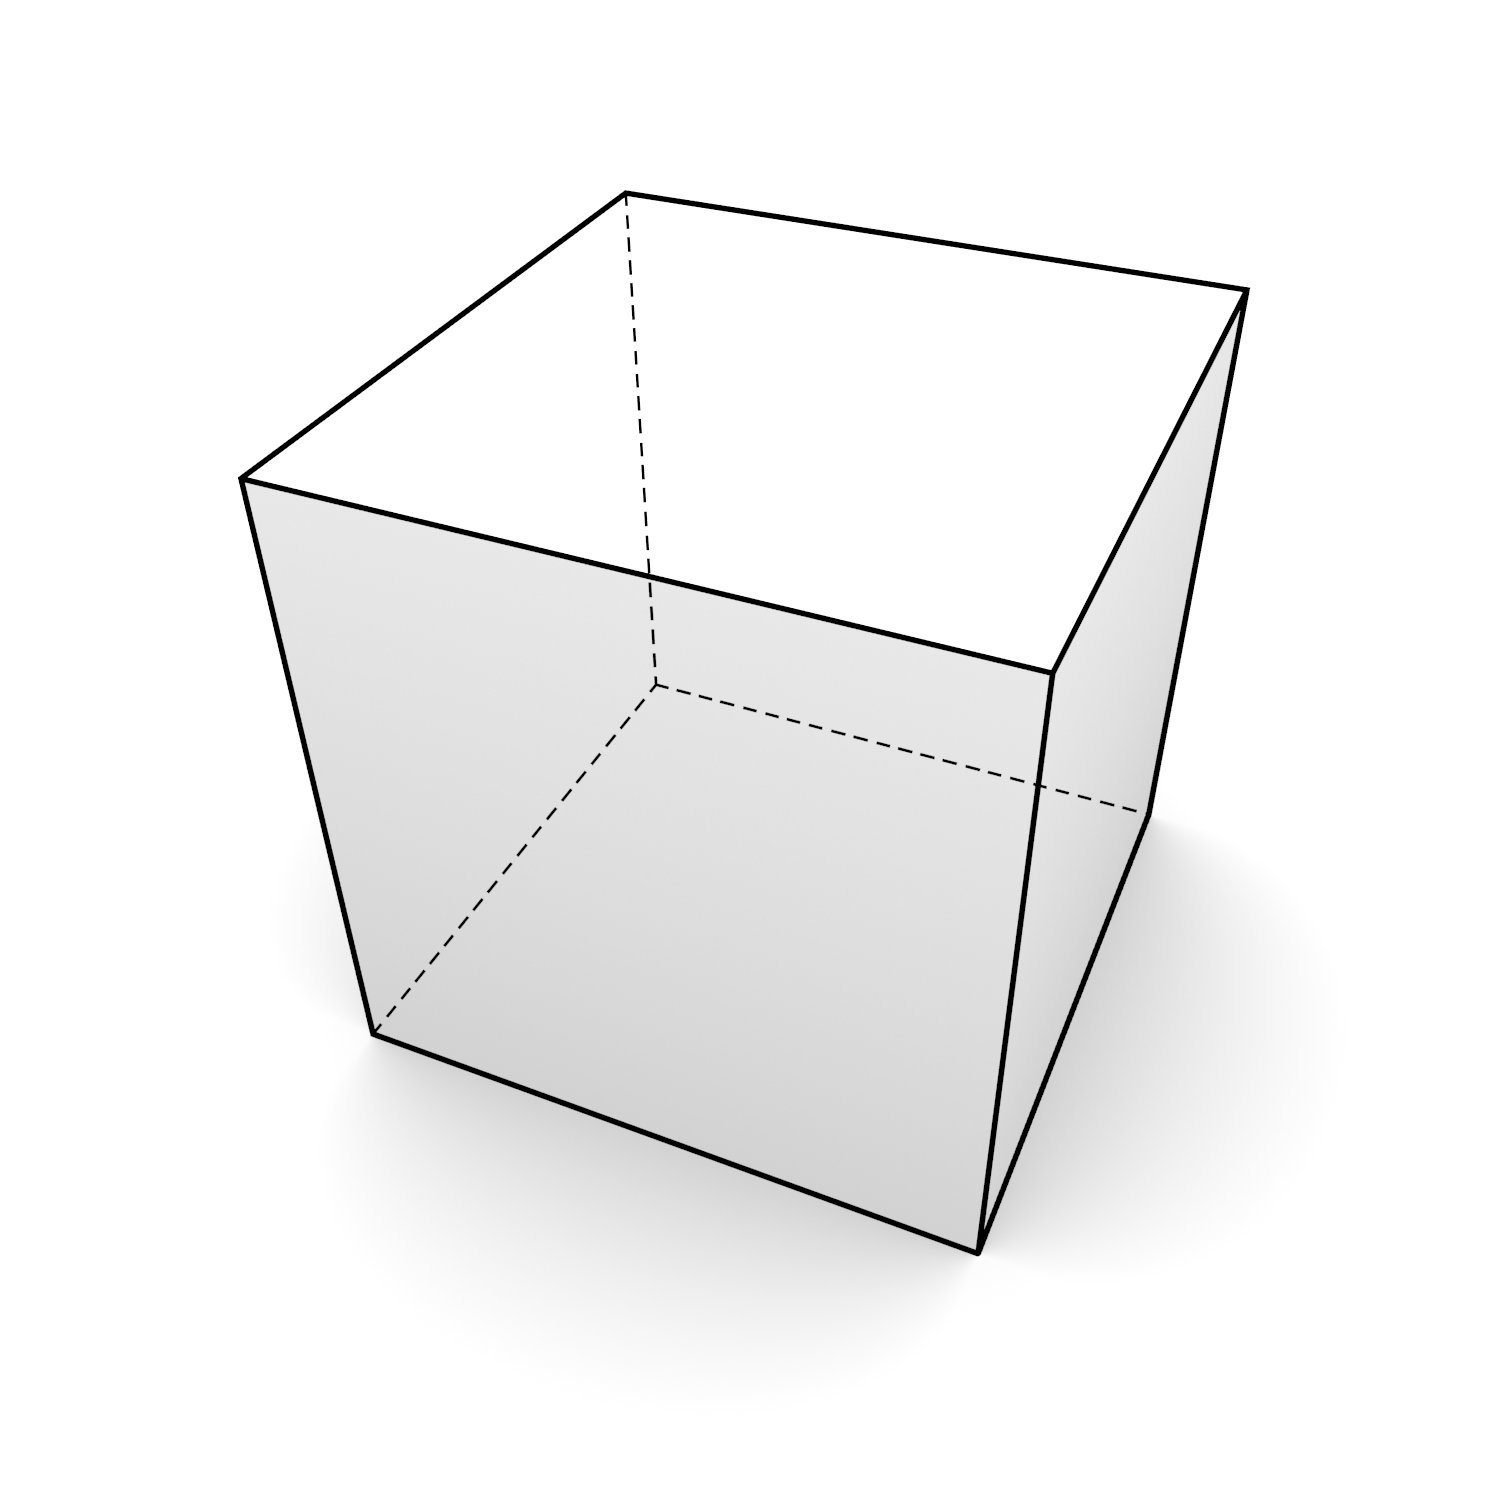
\includegraphics[width=\textwidth]{07-no_overlaps}
    \caption{\note{info}}
    \label{fig:bend-matrix:1}
  \end{subfigure}
  \begin{subfigure}[b]{0.49\textwidth}
    \centering
    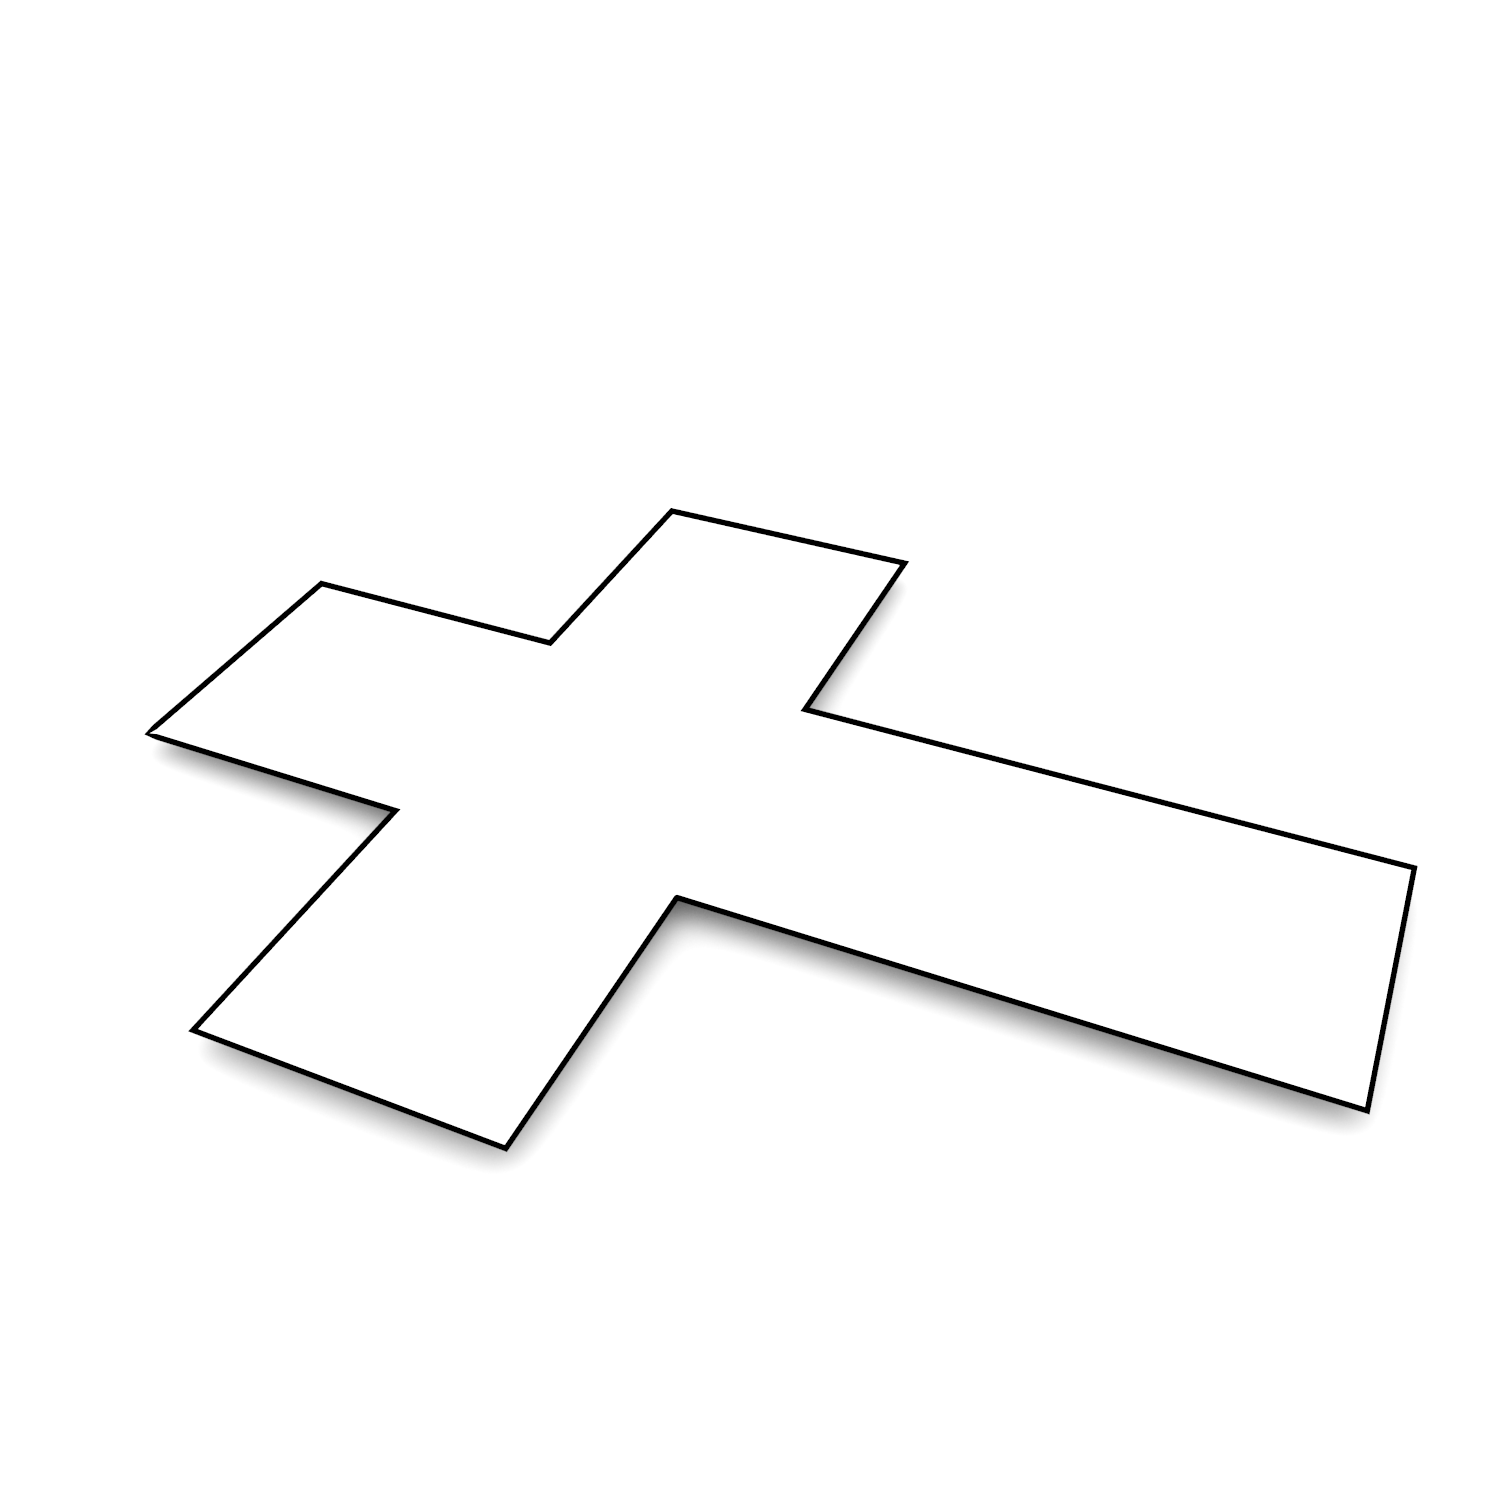
\includegraphics[width=1\textwidth]{07-no_overlaps_2d}
    \caption{\note{info}}
    \label{fig:bend-matrix:2}
  \end{subfigure}
  \begin{subfigure}[b]{0.49\textwidth}
    \centering
    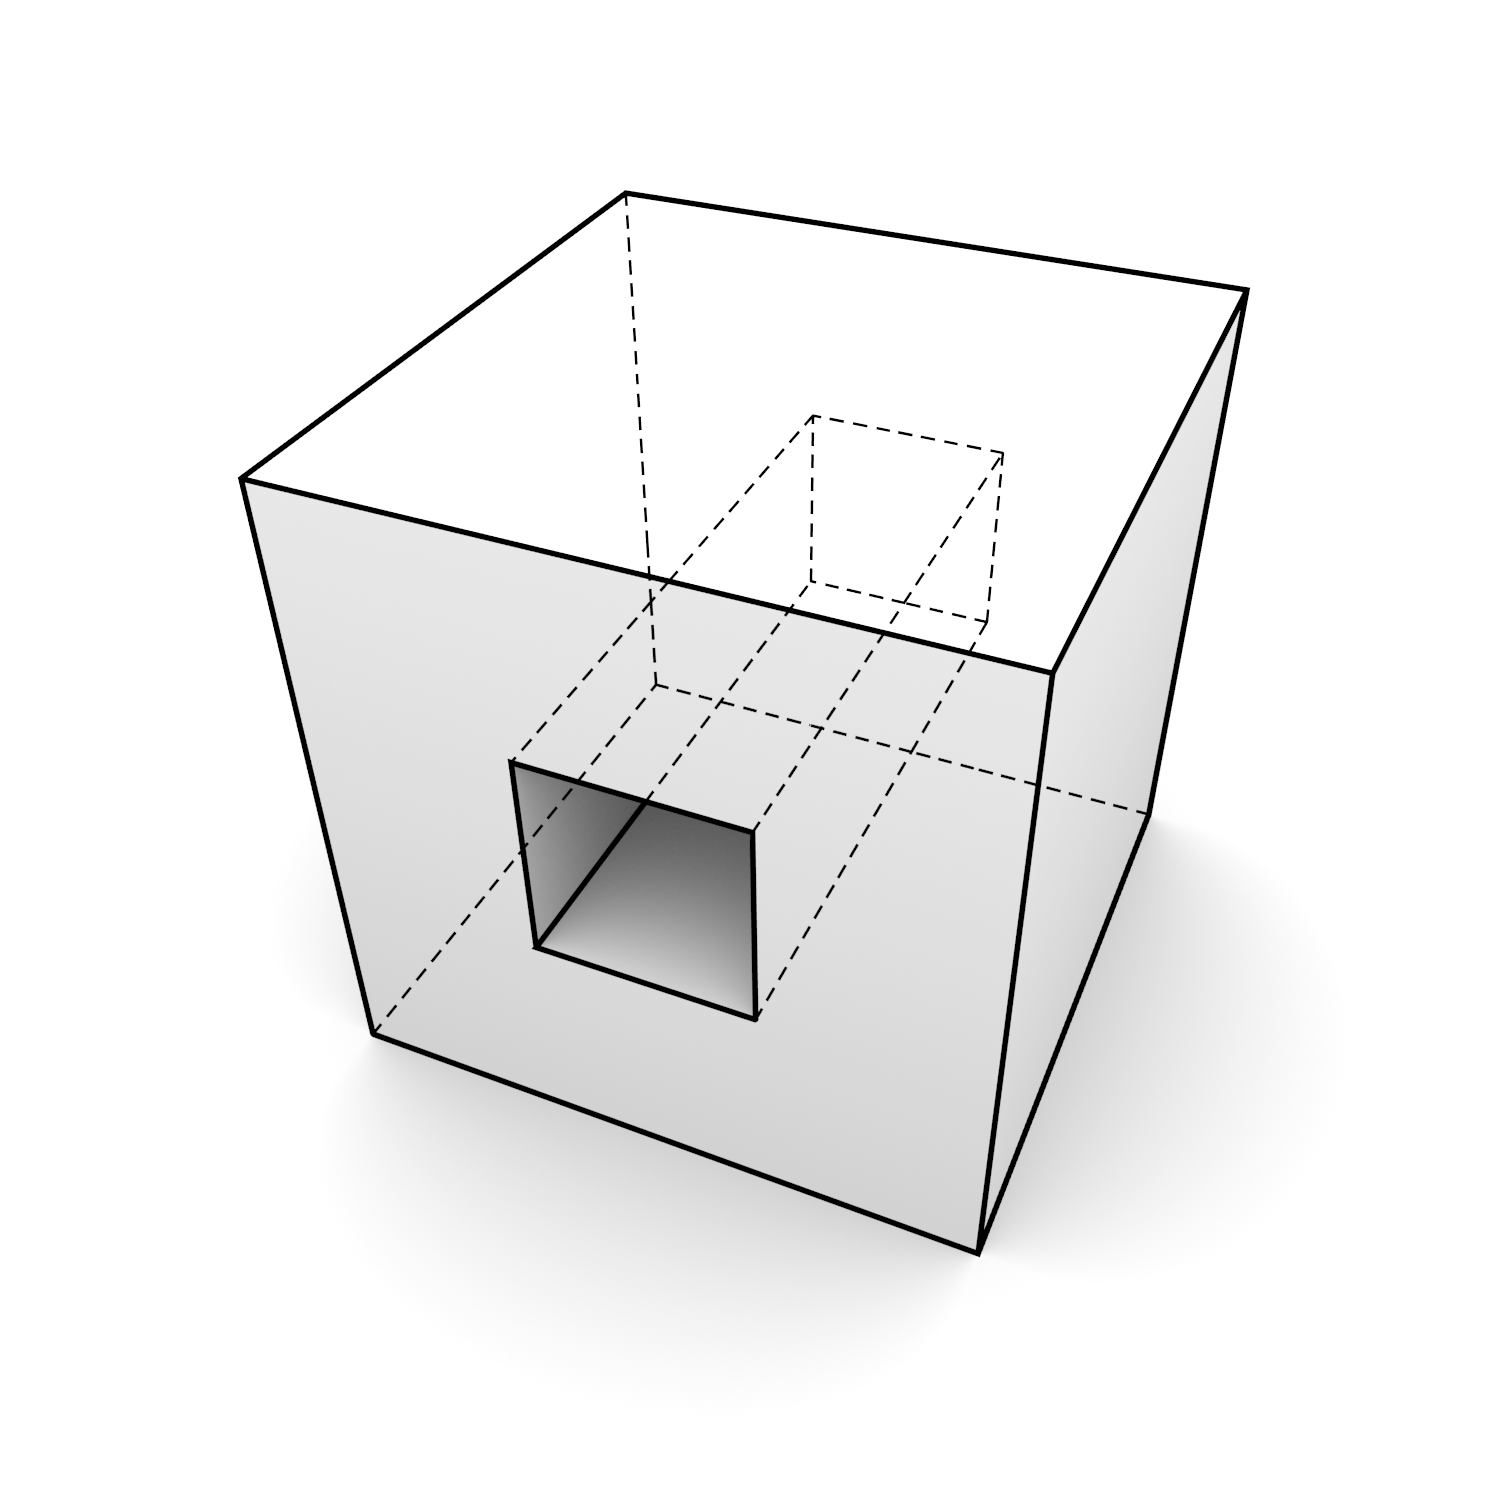
\includegraphics[width=\textwidth]{07-overlaps}
    \caption{\note{info}}
    \label{fig:bend-matrix:3}
  \end{subfigure}
  \begin{subfigure}[b]{0.49\textwidth}
    \centering
    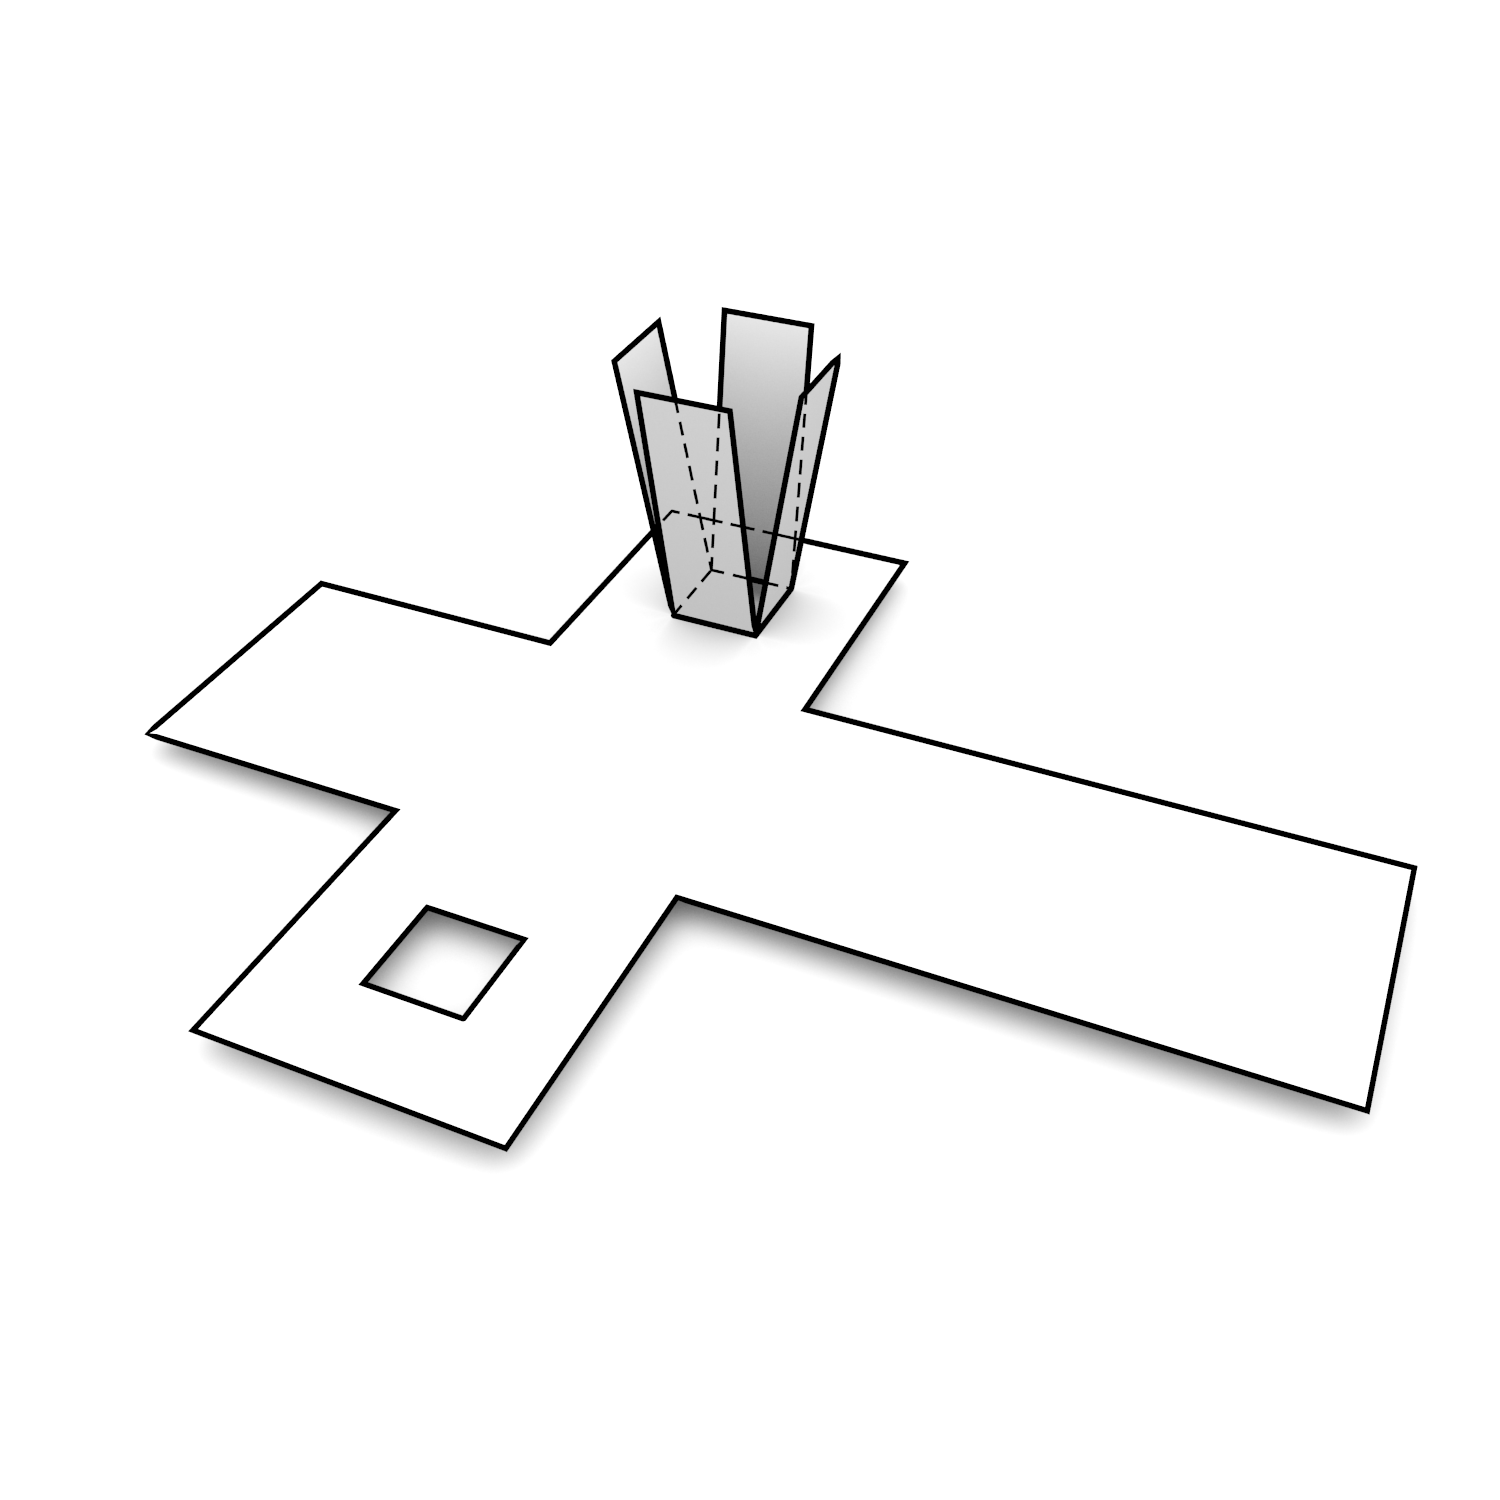
\includegraphics[width=1\textwidth]{07-overlaps_2d}
    \caption{\note{info}}
    \label{fig:bend-matrix:4}
  \end{subfigure}
  \caption{\note{how the bend matrix is created}}
  \label{fig:bend-matrix}
\end{figure}

\begin{listing}[ht]
\begin{minted}[
linenos,breaklines
]{coffeescript}
angle = (180 - connection.parameters.angle) * Math.PI / 180
intersectionLine = connection.parameters.intersectionLine
start = intersectionLine.start.clone()

lineDir = plate.shape.normal.clone().cross connection.node.shape.normal
end = start.clone().add lineDir

start = start.applyMatrix4 rotMat
end = end.applyMatrix4 rotMat

axis = start.clone().sub end
axis.normalize()

moveMat1 = new THREE.Matrix4().makeTranslation(
  -start.x,
  -start.y,
  -start.z
)
moveMat2 = new THREE.Matrix4().makeTranslation start.x, start.y, start.z
bendMat = new THREE.Matrix4().makeRotationAxis axis, angle

newRotMat = moveMat2.clone().multiply bendMat
newRotMat = newRotMat.multiply moveMat1
newRotMat = newRotMat.multiply rotMat.clone()
\end{minted}
\caption{Creating the transformation matrix for a plate as part of a bent plate.}
\label{lst:bend-matrix}
\end{listing}

\section{Alternative solutions}

\subsection{Check for best solution}

The current implementation does not always find the best solution. While traversing the graph it is possible that there multiple different paths which result in unequally well sets of bent plates. One path could be cut by another via an overlap but the better solution would be if the second path along the graph would cut the first. Because the currently only one attempt to traverse the graph is made the second possibility would not be found.
To avoid this a possible solution is the following: If one plate that should be added to a bent plate but overlaps with one other plate of the bent plate to also check if removing the older plate (and the only via this plate connected plates) and add the new plate results in a better solution.
This will increase the run time and will only result in better solutions for models where the bendable parts of the \threedmodel{} form a highly connected graph.

\subsection{Curved joints}

In the current implementation the finger joints are generated just based on the plates but not on the bent plates. This means if multiple small plates which each have to small edges to place finger joints on them, the bent plate generated from them would not get Finger joints too.

To avoid this, a new method must be found to generate finger joints at curved edges, because the edge of the plate that connects to the bent plate  will be curved. Additionally the finger joints has to be regenerated for every attempt to add a new plate to a bent plate to check for overlaps because adding plates will change the generated joints.

\subsection{More bend line types}

The current implementation generates independent of the used material a dashed line as bend line. But This is good for paper to fold it there. For acrylic it would be possible to generate a not dashed line that will be engraved to just give a bending hint without weaken the material to much. For wood, on the other side, living hinges should be generated to make the wood bendable at all.


\end{document}